% verslag mod2B
\documentclass{article}
%table of contents
\usepackage[utf8]{inputenc}
\usepackage{url} %nodig om underscores toe te staan in url

%meer ams meer beter

\usepackage{amsmath}
\usepackage{amssymb}
\usepackage{amsthm} %nodig voor blokje
\usepackage{bbm} %indicator
\usepackage{color}

\usepackage{marginnote}
\usepackage[margin=1in,footskip=0.25in]{geometry} %heb wat meer ruimte

%Plaatjes
\usepackage{graphicx}
\usepackage{float}
\usepackage{caption}
\usepackage{subcaption}
\usepackage{epstopdf}
\usepackage{import} % handig bij importeren van dingen uit andere mapjes
\usepackage{wallpaper} %voorblad
\usepackage{wrapfig} %plaatjes in tekst

\newcommand*{\blankpage}{%
\vspace*{\fill}
{\centering This page is left intentionally blank.\par}
\vspace{\fill}}
\newcommand{\orde}[1]{\mathcal{O}(#1)}
\newcommand{\Z}{\mathbb{Z}}
\newcommand{\R}{\mathbb{R}}
\newcommand{\C}{\mathbb{C}}
\newcommand{\Q}{\mathbb{Q}}
\newcommand{\N}{\mathbb{N}}
\newcommand{\ceiling}[1]{\lceil #1 \rceil}
\newcommand{\floor}[1]{\lfloor #1 \rfloor}


\begin{document}

When the location of each celestial body is determined, one can calculate their velocities, assuming they all move in a uniformal circular orbit.
With this assumption, we have that centripetal force on each body $i$ is exactly the gravitational force, with:
\begin{align*}
F_{centr,i} &= \frac{m_i\cdot v_i^2}{r_i^2}\\
F_{grav, i} &= G\cdot \frac{m_i\cdot M}{r_i}
\end{align*}
where $m_i$ the mass of body $i$, $v_i$ the velocity of body $i$, $r_i$ the distance between body $i$ and the star, $G$ the gravitation constant and $M$ the mass of the star.
As a result of these formulas, the absolute value of the circular velocity $v_i$ of body $i$ is given by:
\begin{align*} 
v_i^2 = \frac{G\cdot M}{r_i}
\end{align*}

\begin{wrapfigure}{r}{0.2\textwidth}
\vspace{-30pt}
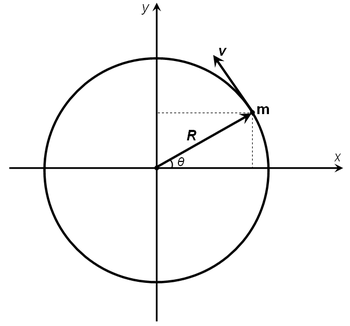
\includegraphics[scale=0.4]{cirkelbaan.png}
\caption{Orbit}
    \label{fig:cirkelbaan}
\end{wrapfigure}

Thereafter, we need to find the velocity in the two dimensions.
Here we assume that each body's orbit is leftwise (see Figure \ref{fig:cirkelbaan}.).
This means that each body has a radius $r$ and an angular velocity $\omega$ such that:
\begin{align*}
\vec{x}(t) = \begin{pmatrix}
R \cos(\omega t)\\
R \sin(\omega t)\\
\end{pmatrix}
\end{align*} 
Thus we have:
\begin{align*}
\vec{v}(t) = \begin{pmatrix}
-R \omega \sin(\omega t)\\
R \omega \cos(\omega t)\\
\end{pmatrix} = \begin{pmatrix}
-\omega x_2(t)\\
\omega x_1(t)\\
\end{pmatrix}
\end{align*} 
As a consequence, we find that $v_1$ is proportional to $-x_2$ and $v_2$ to $x_1$.
With this result we can calculate the initial values of the velocities of the celestial bodies.




\end{document}


